
\part{燃烧与燃烧室}

\begin{tcolorbox}
    针对常用的航空燃气涡轮发动机,请回答并分析以下问题:
    \begin{enumerate}
        \item 请以一款典型航空燃气涡轮发动机为例(可参考 CFM56,GE90,F119,M88
        ,EJ200, RB199, AL-31F 等),说明主燃烧室和加力燃烧室的燃烧组织技术,包括
        但不限于诸如扩压、火焰稳定、燃油喷射、流量分配、混合的设计方法与形式。
        \item 分析总结主燃烧室与加力燃烧室在设计中的异同;
        \item 总结近五十年来国际国内主燃烧室和加力燃烧室的出口温度水平与推力水平,
        并图示。
    \end{enumerate}
\end{tcolorbox}

\section{第一题}

本节以 CFM56 为例简单介绍燃烧室中的燃烧组织技术。
CFM56 是 CFM 国际公司设计的一款高涵道比涡轮风扇发动机,是世界上使用最广泛的涡扇发动机之一,安装于波音 737 及空中客车 A320 等客机上。

\begin{figure}[!ht]
    \centering
    \begin{subfigure}{0.5\linewidth}
        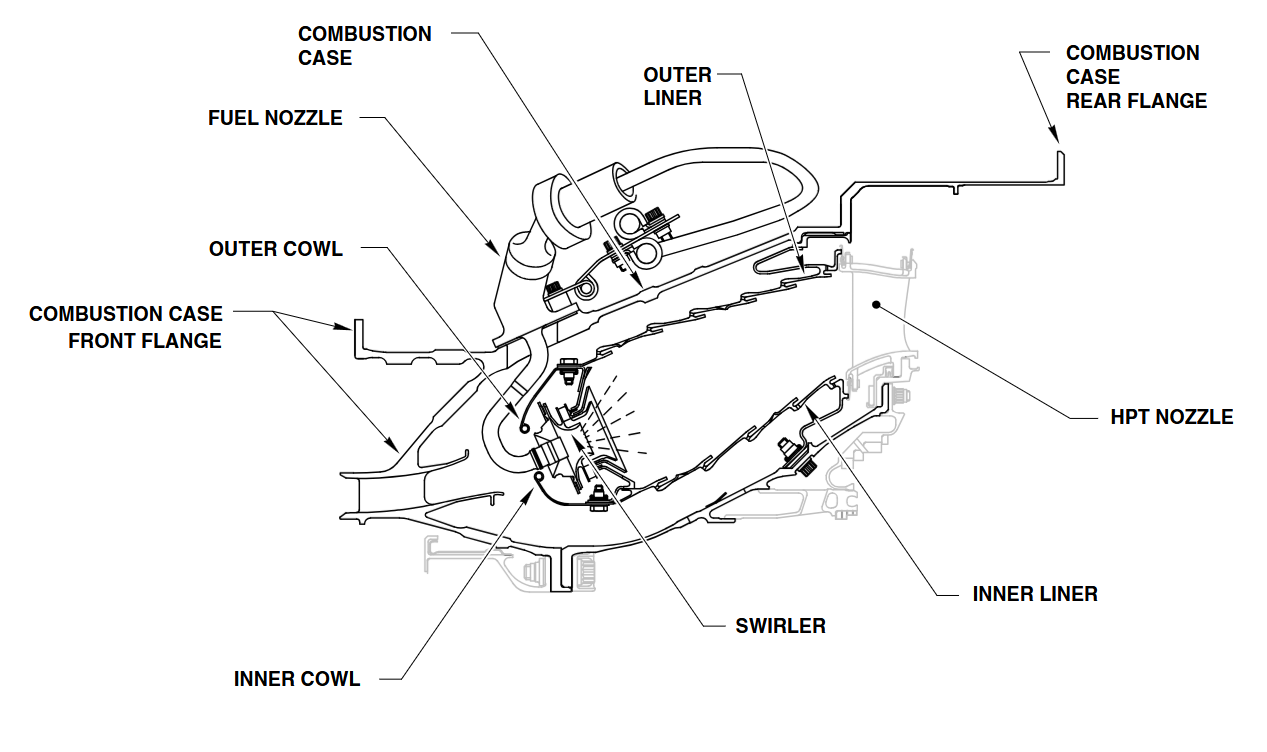
\includegraphics[width=\linewidth]{combustor-1.png}
        \caption{单环形燃烧室}
    \end{subfigure}
    \hfil
    \begin{subfigure}{0.45\linewidth}
        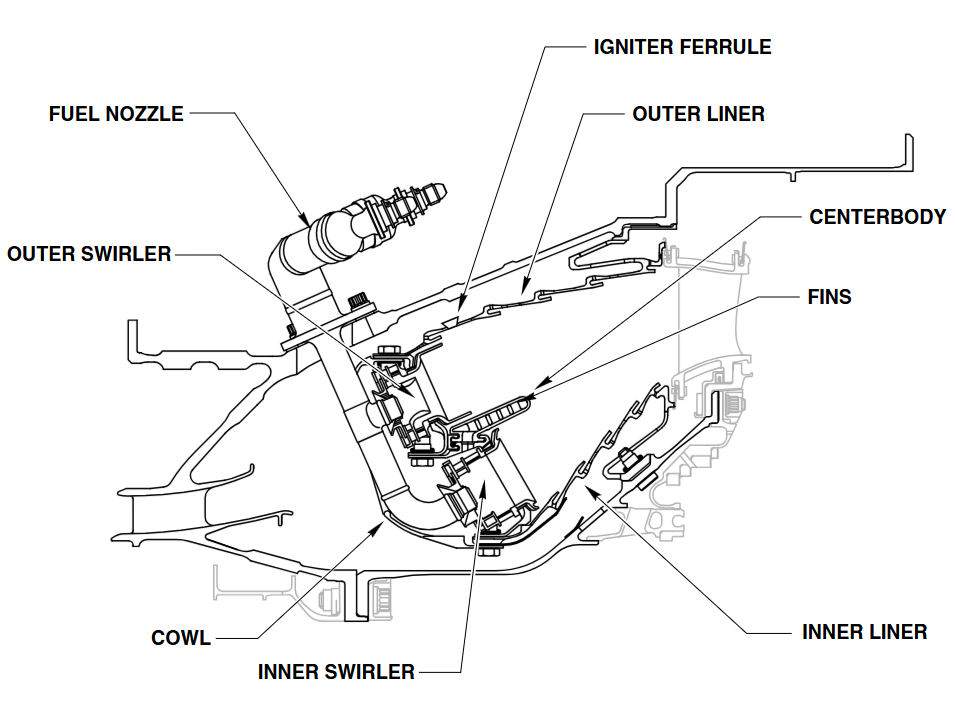
\includegraphics[width=\linewidth]{combustor-2.png}
        \caption{双环形燃烧室}
    \end{subfigure}
    \caption[CFM56 中使用的两种燃烧室截面图。]{CFM56 中使用的两种燃烧室截面图。}
    \label{fig:part-3-combustor}
    \textit{\small 来源:CFM56 维护训练手册 \\ (TRAINING MANUAL CFM56-ALL BORESCOPE INSPECTION)}
\end{figure}

CFM56 上只安装了一个主燃烧室,其有多种设计方式,包括管形燃烧室或环管形燃烧室等,但是安装最广泛的版本使用的是环形燃烧室。
其上安装的环形燃烧室也分为单环形燃烧室和双环形燃烧室两种,主流的燃烧室设计是前者,而双环形燃烧室则可在高推力工况下使用双燃烧室,从而降低污染物的排放。

扩压器(Diffuser)是在燃烧室之前通过降低气体流速以提高压强的部件,在图~\ref{fig:part-3-combustor}中体现为入口后燃烧室腔的突然膨胀,这种扩压器称为突扩扩压器(Step diffuser)。
部分燃烧室的进气道会在气体流动方向上扩张,这种扩压器称为前置扩压器(Prediffuser)。
扩压可将压气机出口的气体中的动压恢复为静压,从而降低燃烧室的压力损失并缩小燃烧室的长度,提高燃烧效率。
另一方面,由于部分高速空气需从火焰筒上的孔中通过射流掺混,未经扩压的空气静压不足,会影响空气流量,从而影响燃烧。
针对扩压器的设计,一般要求其压力损失低、长度短、前置扩压器无分离、出口气流在周向和径向均匀、在所有工况下运行稳定且对压气机出口流场变化不敏感。

\begin{figure}[!ht]
    \centering
    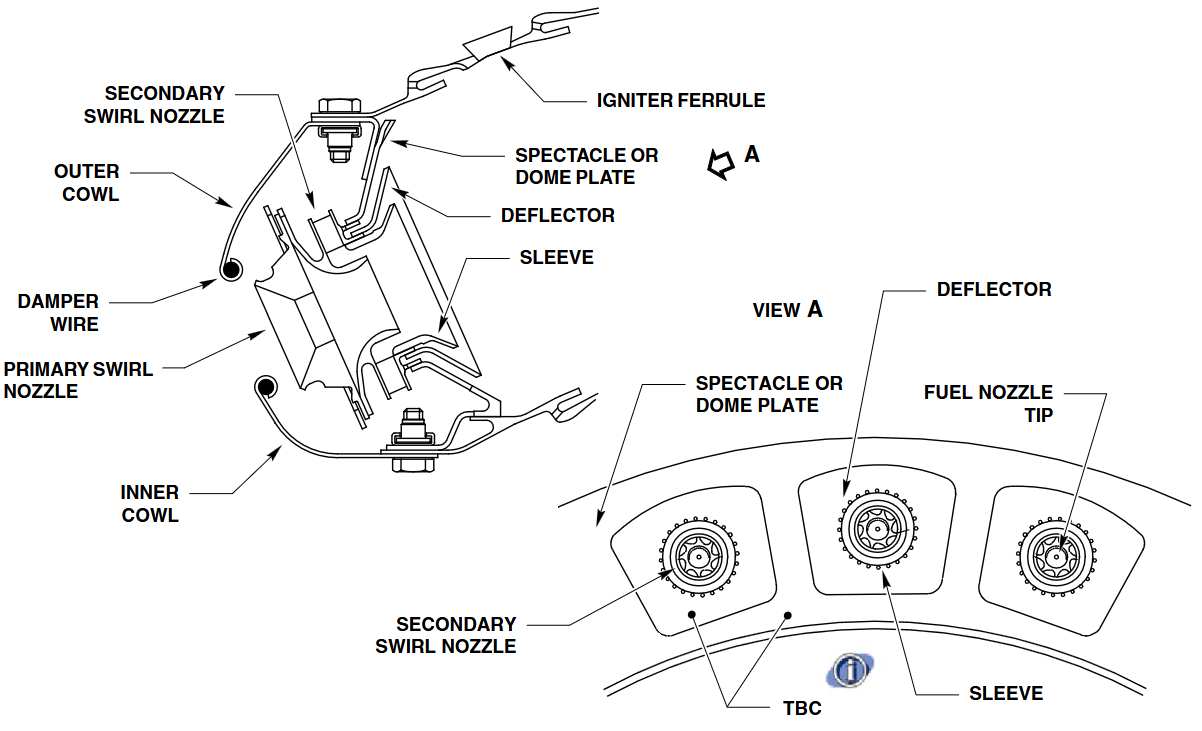
\includegraphics[width=0.8\linewidth]{combustor-nozzle.png}
    \caption{CFM56 单环形燃烧室喷嘴附近细节图。}
    \label{fig:part-3-combustor-nozzle}
    \textit{\small 来源:CFM56 维护训练手册}
\end{figure}

火焰稳定性是燃烧室设计的重要指标之一,而影响火焰稳定的重要参数是主燃区中,即紧邻燃料喷嘴的燃烧区域中,的空气流动。
通过操作空气流动以保证火焰稳定的主要方式是在喷嘴周围安装旋流器(Swirler,参见图~\ref{fig:part-3-combustor}),在主燃区形成回流区。
旋流器有径向和轴向两种设计方式,在此基础上还有多级的旋流器设计。
如图~\ref{fig:part-3-combustor-nozzle}所示,CFM56 燃烧室中的旋流器采用两级设计,并同时承担燃料喷嘴和雾化的功能,主旋流器直接从轴向进气,而副旋流器则从侧向进气。
旋流器能够使气流高速旋转,产生强旋流流场,从而在旋流器出口附近形成一块空气反向流动的区域,称为回流区。
回流的气体中充满高温燃烧产物,因此可提供自动点火源,维持火焰稳定;此外,回流区中还具有流动速度较低的低速区。
因此,在回流区内进行的燃烧因此具有较好的火焰稳定性以及混合效果。

\begin{figure}[!ht]
    \centering
    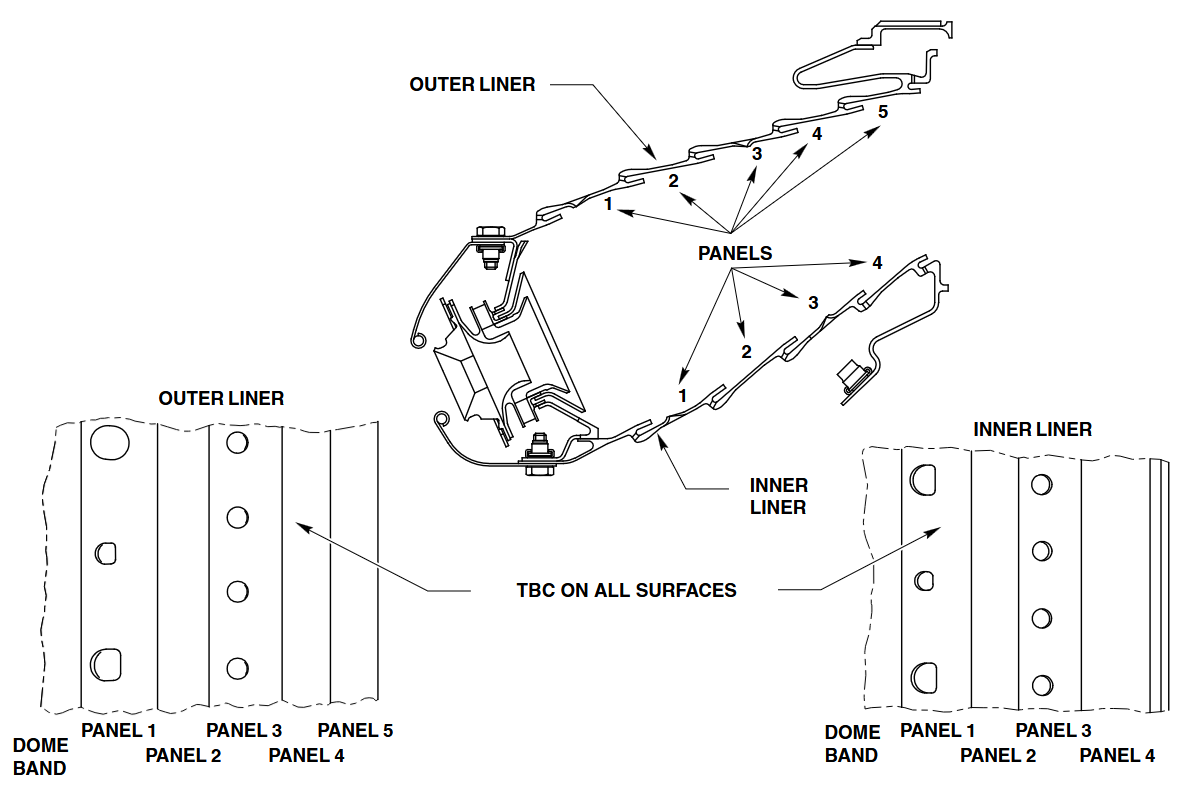
\includegraphics[width=0.8\linewidth]{combustor-liner.png}
    \caption{CFM56 单环形燃烧室火焰筒细节图。}
    \label{fig:part-3-combustor-liner}
    \textit{\small 来源:CFM56 维护训练手册}
\end{figure}

空气除了经过旋流器和燃料喷嘴进入燃烧室火焰筒外,还可通过火焰筒上的小孔形成射流而进入火焰筒并参与燃烧。
根据射流形成的位置,可将其分为在主燃区中的主燃孔射流和在主燃区外的掺混射流两种。
主燃孔射流可补充主燃区中回流区的流动、调整主燃区的油气比并改善火焰稳定,降低污染排放物,缩短回流区并强化燃烧过程。
此外,射流还能调整径向温度分布并减少热点。
通过孔的射流会孔的几何结构、环腔高度和压力参数等因素的影响。
图~\ref{fig:part-3-combustor-liner}中可见 CFM56 火焰筒上孔洞的组织,其中掺混射流使用简单平圆圆孔,而主燃孔射流部分使用单卷边孔。
单卷边孔的穿透角度更大,有利于主燃孔射流缩短回流区流动,从而提高燃烧效率。

空气流量分配是燃烧室中燃烧组织的重要部分,进入燃烧室的空气按用途可分为旋流器气量、头部冷却气量、主燃孔气量、掺混气量和火焰筒冷却气量。
其中,进入旋流器、用于头部冷却和通过主燃孔的气量,以及在主燃区中通过火焰筒上平行于轴向的通道冷却火焰筒的气流均可参与主燃区的燃烧。
这些气量统称主燃区空气流量,而这些空气占所有空气流量的比值是一个重要的参数,通常是通过设计点油气比,即整个燃烧室的油气比,和主燃区油气比确定的。
主燃区油气比的选择很大程度上取决于燃烧室的设计指标。
根据主燃区油气比和化学恰当油气比($F_\text{st} = 0.068$)之间的关系,可将主燃区分为富油、化学恰当和贫油主燃区三种。
富油主燃区在小功率情况下效率较高,且能较容易地实现高空重点火,但是燃烧效率较低,污染严重;
相对地,贫油主燃区大功率情况下燃烧效率较高,冷却较好且出口温度分布优良,但是稳定性和点火性能较差。

通常用于民用航空器的 CFM56 发动机不具有加力燃烧室,但对加力燃烧室中的燃烧,需要将外涵道含氧量更高的低温空气与内涵道低氧高温空气混合,在克服低氧浓度的同时利用高温空气组织燃烧。
在加力燃烧室中,空气的混合一般是和扩压同时进行的。

\section{第二题}

主燃烧室和加力燃烧室的工况和设计要求不同,因此采用了不同的设计方式。
相较于主燃烧室,加力燃烧室的进口总压更低而温度更高,进口空气速度更高而含氧量更低。
和两者之间工况的差距巨大这一情况不同,主燃烧室和加力燃烧室的设计性能要求是比较接近的,均需要较高的燃烧效率以及燃烧稳定性和较低的压降损失。
在这些设计指标的要求下,两者自然具有相对不同的设计特点。
主燃烧室需要降低进口速度以恢复动压头;进行燃油雾化以强化燃烧过程;利用低速区或回流区稳定火焰并通过空气分股稳定火焰且调整温度分布。
加力燃烧室则通过降低进口速度并将内外涵道气流混合以减少加热损失,降低总压损失;进行燃油雾化以强化燃烧过程;利用低速区或回流区稳定火焰;并利用外涵道较冷的气流冷却外壳。

根据这些设计特点,主燃烧室和加力燃烧室的主要组成也不同。
主燃烧室一般由机匣、扩压器、火焰筒、火焰稳定器(旋流器)和燃油喷嘴几个部分组成。
机匣是发动机的承力件;
扩压器将压气机出口空气流的速度降低以回复压头;
火焰筒用来控制燃烧和掺混空气射流以及冷却空气膜;
旋流器安装在燃烧室头部的,产生稳定火焰的旋流或者涡;
喷嘴则为主燃区提供燃料。
相对的,加力燃烧室通常由扩压器或混合器、燃油喷射器、点火器、稳定器和冷却火焰筒组成。
扩压器用于涡轮喷气式发动机的加力燃烧室,可降低流速,提高静压;
而混合器则用于涡轮风扇发动机,可混合核心机高温热气流与外涵气流;
燃油喷射器和点火器分别用于添加燃料以及点火,由于工况不同,加力燃烧室中的喷射器和点火器设计也与主燃烧室中的不同;
稳定器用于控制气流以提供稳定燃烧的环境,加力燃烧室中通常不使用旋流器,而是使用被动的设计,如沙丘驻涡稳定器;
由于工作温度更高,加力燃烧室中的火焰筒冷却也与主燃烧室不同,通常采用面积更大、流量更少的冷却方式。

\section{第三题}

针对特定型号的引擎的主燃烧室和加力燃烧室的出口温度以及推力水平较难查找。
对主燃烧室的出口温度,我们使用涡轮进气温度(Turbine Inlet Temperature)近似。
数据总结在表~\ref{tab:combustors}和图~\ref{fig:combustors}中。
总体而言,近五十年来各型号涡轮发动机的主燃烧室出口温度、正常推力和加力推力都呈上升趋势。

\begin{table}[!ht]
    \centering

    \caption{近五十年航空引擎燃烧数据对比}
    \label{tab:combustors}
    \makebox[\textwidth]{
        \begin{tabular}{cccccc}
            \hline
            产品名 & 原产地 & 年份 & 进气温度(\unit{\degreeCelsius}) & 正常推力(\unit{kN}) & 加力推力(\unit{kN}) \\ \hline
            J57 & 美国 & 1950 & 870 & 52.0 & 76.5 \\
            J79 & 美国 & 1955 & 935 & 52.8 & 80.0 \\
            R-11 & 苏联 & 1956 & 955 & 38.7 & 60.6 \\
            TF30 & 美国 & 1960 & 1170 & 64.8 & 111.7 \\
            AL-21F & 苏联 & 1966 & 1100 & 76.4 & 109.8 \\
            R-29 & 苏联 & 1972 & 1083 & 78.5 & 112.8 \\
            M52 & 法国 & 1974 & 1327 & 64.0 & 95.0 \\
            AL-31F & 苏联 & 1981 & 1392 & 76.5 & 122.6 \\
            F119 & 美国 & 1986 & 1649 & 116.0 & 156.0 \\
            M88 & 法国 & 1986 & 1577 & 50.0 & 75.0 \\
            AL-41F & 苏/俄 & 2001 & 1642 & 117.6 & 176.4 \\
            涡扇-15 & 中国 & 2006 & 1568 & 105.0 & 156.0 \\
            F135 & 美国 & 2009 & 1980 & 125.0 & 191.0 \\
            \hline
        \end{tabular}
    }
\end{table}

\begin{figure}[!ht]
    \centering
    \begin{subfigure}{0.9\linewidth}
        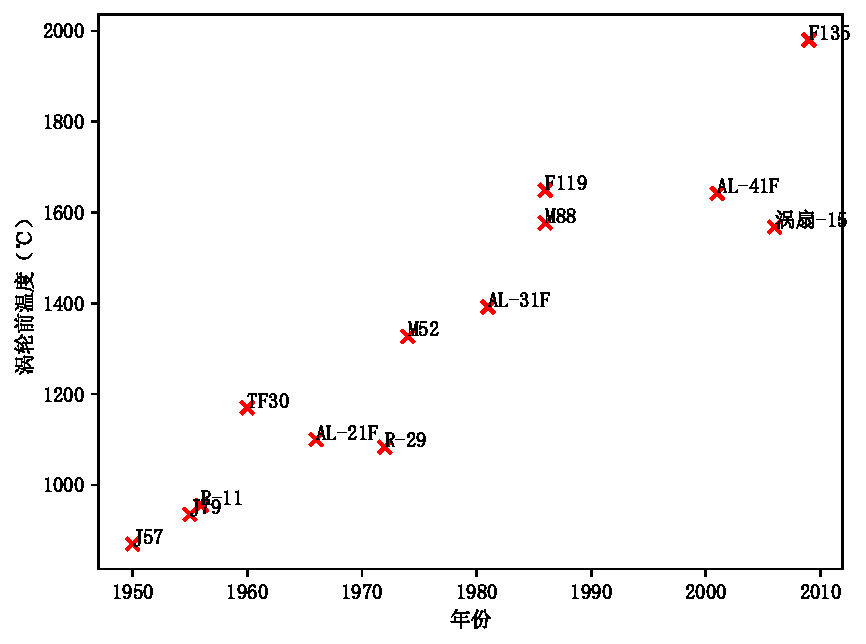
\includegraphics[width=\linewidth]{combustor-tit.pdf}
    \end{subfigure}

    \begin{subfigure}{0.9\linewidth}
        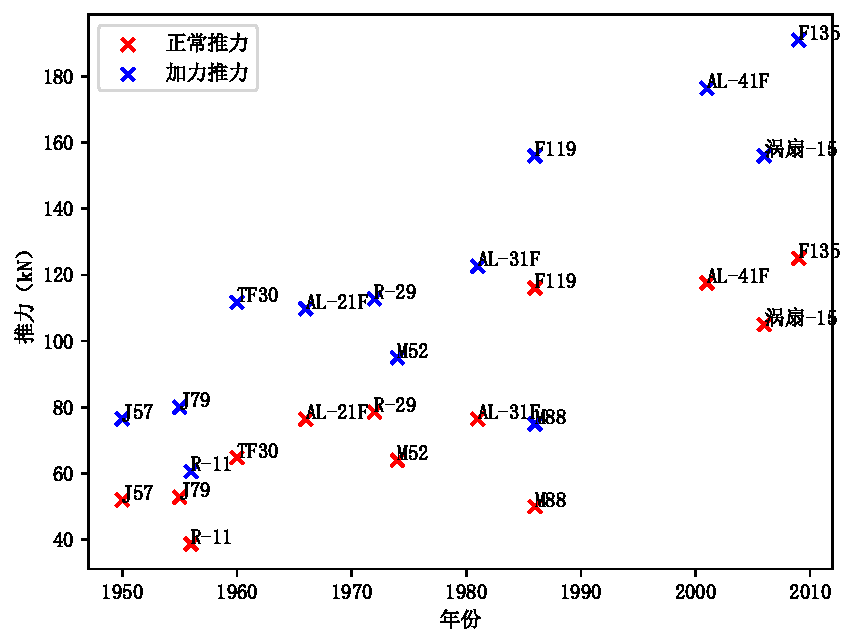
\includegraphics[width=\linewidth]{combustor-thrust.pdf}
    \end{subfigure}
    \caption{近五十年航空引擎燃烧数据对比。}
    \label{fig:combustors}
\end{figure}

